\chapter{Reversibility \& The Arrow of Computation}

\section{\textbf{Why computation moves forward, and what ``forward'' even means.}}

Throughout the previous section of this book, we have constructed a rigorous geometry of computation. We have defined **worldlines** as the specific paths taken through the graph, **bundles** as the clustering of legal possibilities, **interference** as the shaping force that constraints those possibilities, and **collapse** as the decisive mechanism of choice[cite: 1, 2].

Now, however, we must confront a deeper, more existential question that arises from these mechanics:

\begin{quote}
\textbf{Why does computation move forward? Why is there an ``arrow'' at all? Why can we collapse bundles into a worldline but never ``un-collapse'' them? Why does time in computation feel irreversible?}
\end{quote}

It is crucial to understand that this is not a question of physics[cite: 3]. We are not discussing thermodynamics or entropy in the material sense. It is a computational question, and the answer derives directly from the structure of the Recursive Metagraph (RMG) universe itself[cite: 3]. Let us make this precise and sane[cite: 4].

\begin{center}\rule{0.5\linewidth}{0.5pt}\end{center}

\section{\texorpdfstring{\textbf{Rewrites Are Directional}}{14.1 --- Rewrites Are Directional}}

The fundamental unit of change in our system is the Double-Pushout (DPO) rewrite. Every single rewrite is composed of three distinct elements: an **L** pattern which marks the structure to be deleted, a **K** interface which marks the structure to be preserved, and an **R** pattern which marks the structure to be created[cite: 5].

This tripartite structure inherently defines a vector: a movement from **Before** to **After**. This is not necessarily ``forward in time'' in a temporal sense, but it is distinctly ``forward in structure''[cite: 6].

Consider the asymmetry of the operation. Deletion breaks information symmetry by removing connections, while insertion adds new, specific asymmetry to the graph[cite: 6]. Preservation stabilizes the continuity between these two states. The triple $(L,K,R)$ creates a definitive direction[cite: 6]. You cannot spontaneously reconstruct the deleted structure ($L \setminus K$) from the created structure ($R \setminus K$) without possessing extra, external information[cite: 7]. That structural asymmetry is the origin of \textbf{the arrow}[cite: 7].

\begin{figure}[h]
\centering
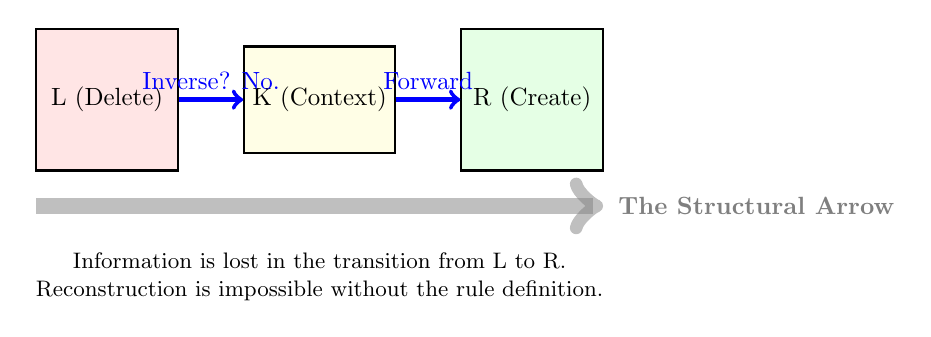
\begin{tikzpicture}[scale=0.9, transform shape]
    % Boxes
    \node (L) [rectangle, draw, thick, minimum width=2cm, minimum height=2cm, fill=red!10] at (0,0) {L (Delete)};
    \node (K) [rectangle, draw, thick, minimum width=1.5cm, minimum height=1.5cm, fill=yellow!10] at (3,0) {K (Context)};
    \node (R) [rectangle, draw, thick, minimum width=2cm, minimum height=2cm, fill=green!10] at (6,0) {R (Create)};
    
    % Arrows
    \draw[->, ultra thick, blue] (L) -- (K) node[midway, above] {Inverse? No.};
    \draw[->, ultra thick, blue] (K) -- (R) node[midway, above] {Forward};
    
    % The Arrow
    \draw[->, line width=2mm, gray, opacity=0.5] (-1, -1.5) -- (7, -1.5) node[right, black] {\textbf{The Structural Arrow}};
    
    % Annotation
    \node[align=center, font=\small] at (3, -2.5) {Information is lost in the transition from L to R.\\ Reconstruction is impossible without the rule definition.};
\end{tikzpicture}
\caption{The Asymmetry of Rewrites: The transition from L to R via K is directional. Without storing the specific history of the deletion, the arrow cannot be reversed.}
\end{figure}

\begin{center}\rule{0.5\linewidth}{0.5pt}\end{center}

\section{\texorpdfstring{\textbf{Collapse Narrows Possibility}}{14.2 --- Collapse Narrows Possibility}}

Every time a collapse occurs, the system performs a specific sequence of operations: it selects \emph{one} rewrite, discards the rest, and commits the universe to a new state[cite: 8].

We must reiterate that this is not entropy, nor is it probability or quantum measurement[cite: 9]. It is best described as the **irreversible contraction of the possibility surface**[cite: 10].

Imagine standing in a room with ten doors. Once you step through one and the door locks behind you, you cannot ``go back'' to the state of having ten options unless the rules of the new room explicitly allow it—and most do not[cite: 10]. Even if the pattern $R$ transforms \emph{back} into $L$, the system does not magically recover the bundle of possibilities it once possessed[cite: 11]. You lose possibility, and you lose it permanently[cite: 11]. That loss is the arrow.

\begin{center}\rule{0.5\linewidth}{0.5pt}\end{center}

\section{\texorpdfstring{\textbf{The Observer (Scheduler) Creates Irreversibility}}{14.3 --- The Observer (Scheduler) Creates Irreversibility}}

In the CΩMPUTER framework, the scheduler acts as the observer. Its role is to order rules, resolve conflicts between competing rewrites, enforce legality, pick the minimal rewrite, and eliminate ambiguity[cite: 12].

This ``observer'' function does not merely record the worldline; it actively \textbf{shapes} it[cite: 13]. By breaking ties, resolving overlaps, and pruning possibility, the observer commits the finality of collapse[cite: 14].

Without a scheduler, the evolution of bundles would remain nondeterministic and hazy. With a scheduler, **every collapse becomes irreversible, because the observer's choice becomes structural history**[cite: 15]. The act of choosing cements the path. That is the arrow[cite: 15].

\begin{center}\rule{0.5\linewidth}{0.5pt}\end{center}

\section{\texorpdfstring{\textbf{Reversibility Is Possible --- But Only When The Rules Allow It}}{14.4 --- Reversibility Is Possible --- But Only When The Rules Allow It}}

This is not to say that reversibility is impossible. Not all rewrites are strictly irreversible[cite: 16]. Some rules possess inverses. If a rule-set explicitly contains a rewrite $L \rightarrow R$ and another rewrite $R \rightarrow L$, then your universe theoretically supports **bidirectional motion**[cite: 17].

However, the existence of inverse rules is not enough. Even with them, the **K-invariants** must still hold, legality must be preserved, wormhole interfaces must align perfectly, and the nested RMG structure must agree[cite: 18]. Reversibility requires **deep structural symmetry**[cite: 19]. Most systems simply do not possess this symmetry; they naturally ``flow downhill'' due to curvature[cite: 19].

\begin{center}\rule{0.5\linewidth}{0.5pt}\end{center}

\section{\texorpdfstring{\textbf{Why High-Level Computation Rarely Reverses}}{14.5 --- Why High-Level Computation Rarely Reverses}}

When we look at realistic, high-level computational systems, we see processes like optimizations, simplifications, normalizations, eliminations, and canonicalizations. We see type inference, folding, propagation, evaluation, and compilation. All of these processes share a common trait: they move toward **fewer possibilities**, not more[cite: 20].

Once you inline a function, you cannot ``un-inline'' it without extra data[cite: 21]. Once you lower an Intermediate Representation (IR), you cannot ``un-lower'' it. Once you compile code, you cannot ``un-compile'' it back to its original semantics without losing significant detail[cite: 21].

This is **not** a flaw of compilers[cite: 22]. It is the **arrow of computation**[cite: 22]. It is a structural necessity, not an accident.

\begin{center}\rule{0.5\linewidth}{0.5pt}\end{center}

\section{\texorpdfstring{\textbf{The Arrow Emerges From Geometry}}{14.6 --- The Arrow Emerges From Geometry}}

The central insight regarding the arrow is geometric: **Worldlines advance in the direction that reduces Rulial Distance between the ``current'' state and the ``goal.''**[cite: 23].

This dynamic gives the universe a gradient. Smooth manifolds create gentle arrows, guiding the system softly. Jagged manifolds create sharp arrows, forcing specific paths. Chaotic manifolds create unpredictable arrows[cite: 23].

Curvature directs the flow; constraints narrow it; bundles shape it; and collapse defines the next step[cite: 24]. Just as a surfer surfs the face of a wave—letting gravity and geometry determine their line—computation surfs the geometry of its own manifold[cite: 25]. That flow, that direction, that inevitability is the arrow[cite: 25].

\begin{figure}[h]
\centering
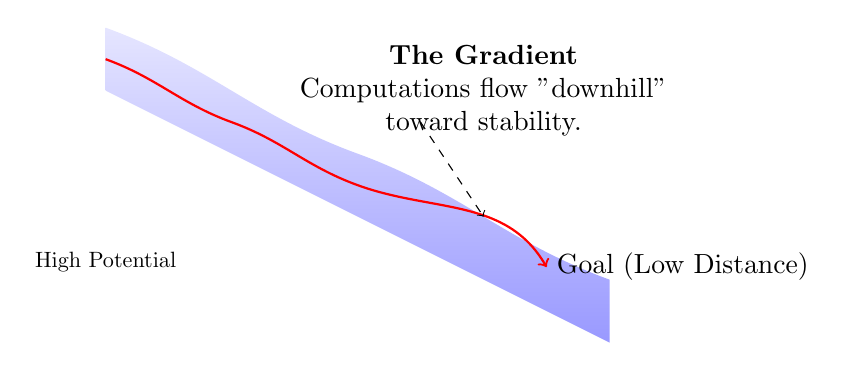
\begin{tikzpicture}[scale=0.8]
    % The Surface
    \shade[top color=blue!10, bottom color=blue!40] (0,4) to[out=-20, in=160] (4,2) to[out=-20, in=160] (8,0) -- (8,-1) -- (0,3) -- cycle;
    
    % The Path
    \draw[thick, red, ->] (0, 3.5) to[out=-20, in=160] (2, 2.5) node[midway, above, black] {High Potential} to[out=-20, in=160] (4, 1.5) to[out=-20, in=120] (7, 0.2) node[right, black] {Goal (Low Distance)};
    
    % Arrow label
    \node[align=center] at (6, 3) {\textbf{The Gradient}\\ Computations flow "downhill"\\ toward stability.};
    \draw[->, dashed] (5, 2.5) -- (6, 1);
\end{tikzpicture}
\caption{The Geometric Arrow: Computation follows the gradient of the manifold, reducing the Rulial Distance to the canonical form.}
\end{figure}

\begin{center}\rule{0.5\linewidth}{0.5pt}\end{center}

\section{\texorpdfstring{\textbf{Forget Physics. The Arrow of Computation Is About Consistency.}}{14.7 --- Forget Physics. The Arrow of Computation Is About Consistency.}}

Irreversibility in CΩMPUTER comes from a confluence of factors: K-interfaces, structural invariants, DPO locality, RMG recursion, collapse rules, scheduling, curvature, and constraint interaction.

It is nothing spooky, mystical, or quantum[cite: 26]. It is simply **overlapping constraints reducing possibility in a structured way**[cite: 27]. This is what makes a worldline \emph{feel} like a timeline[cite: 27].

\begin{center}\rule{0.5\linewidth}{0.5pt}\end{center}

\section{\texorpdfstring{\textbf{Arrow Failure: When Systems Become Reversible By Accident}}{14.8 --- Arrow Failure: When Systems Become Reversible By Accident}}

Reversibility is not always a virtue[cite: 28]. In brittle systems with insufficient pruning, undoing becomes too easy. Contradictory rewrites can oscillate, causing systems to funnel into infinite cycles. In these scenarios, curvature collapses to zero, debugging becomes hellish, and semantics become loose[cite: 29].

We often see this in spaghetti codebases that exhibit the ``reverse wiggle'': you fix a bug, and the system inadvertently returns to its prior broken form via a different rule-chain[cite: 30]. Reversibility is possible—but often undesirable[cite: 30]. The arrow stabilizes computation; its absence destabilizes it[cite: 31].

\begin{center}\rule{0.5\linewidth}{0.5pt}\end{center}

\section{\texorpdfstring{\textbf{Arrow Strength and System Design}}{14.9 --- Arrow Strength and System Design}}

We can characterize systems by the strength of their arrow. Systems with **strong arrows** feel deterministic. They converge toward canonical forms, are easy to optimize, exhibit low curvature, and form stable worldlines. They are, simply put, a joy to work with[cite: 32].

Conversely, systems with **weak arrows** feel chaotic. They loop unpredictably, reintroduce past states, exhibit unstable curvature, and have fragile worldlines. These are the engineering nightmares[cite: 33].

System design is, in part, **the art of giving your universe a healthy, coherent arrow**[cite: 33].

\begin{center}\rule{0.5\linewidth}{0.5pt}\end{center}

\section*{\texorpdfstring{\textbf{FOR THE NERDS™}}{FOR THE NERDS™}}

\section{\texorpdfstring{\textbf{Arrow = Partial Order on RMG States}}{Arrow = Partial Order on RMG States}}

Formally, the arrow is induced by the rewrite relation ($\rightarrow$), which is well-founded under DPO legality[cite: 34]. This creates a partial order on RMG states, where irreversible rewrites generate acyclic progress[cite: 34]. This gives the computational universe a Directed Acyclic Graph (DAG) structure—not within the RMG itself, but in the meta-space of its evolution[cite: 35].

\emph{(End sidebar.)} [cite: 35]

\begin{center}\rule{0.5\linewidth}{0.5pt}\end{center}

\section{\texorpdfstring{\textbf{Transition: Part III Complete}}{14.10 --- Transition: Part III Complete}}

You now possess the complete vocabulary of Part III. You understand **worldlines** as motion, **bundles** as possibility, **interference** as forces, and **collapse** as commitment. You grasp **curvature** as resistance, **local NP collapse** as flattening, and **the arrow** as direction[cite: 36].

This is the physics of computation. You have left the cave and climbed the ridge[cite: 37]. You are now looking at the whole computational universe like a surfer looking at the ocean—reading sets, anticipating breaks, and feeling the deep patterns beneath the surface[cite: 37]. You are ready for Part IV[cite: 38].

Where we build...

\textbf{machines that span universes.}
